\begin{frame}{Introduction}
\begin{itemize}
  \item Collaborative concept mapping
  \item Collaborative concept mapping with KB approach
  \item Challenges
  \item Research objectives
\end{itemize}
\end{frame}


\begin{frame}[allowframebreaks]{Why collaborative learning is important?}

    \begin{figure}[tb]
        \begin{center}
            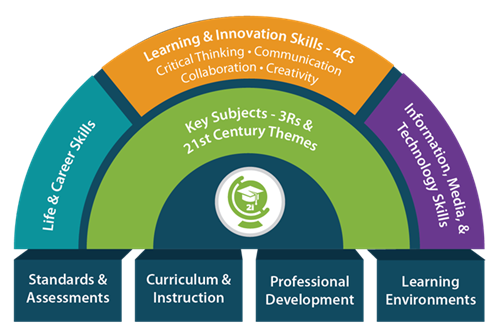
\includegraphics[width=70mm]{images/p21centuryskills.png}
        \end{center}
        \caption{Partnership for 21st century learning. Source: https://www.battelleforkids.org/networks/p21}
        \label{intro::p21}
    \end{figure}

    \begin{itemize}
        \item Collaboration is one of the four-essential skills in 21st century skills
        \item The advancement of technology and rapidly changing environment require 
        collaborative works of multidisciplinary experts to solve complex problems effectively
        \item Collaboration does not merely happen just because individuals are co-present
        \item It is indeed necessary to practice collaboration in the classroom
    \end{itemize}
\end{frame}

\begin{frame}[allowframebreaks]{Designing learning activities to encourage collaboration}
    \begin{itemize}
        \item Students' interactions play a fundamental role in collaborative learning 
        \cite{Baines2009ImprovingStudy,Webb2009TheClassroom}
        \item Various instructional strategies are employed to encourage learners to collaborate 
        (i.e. scripts, scenarios, representational tools).
        \item During collaboration individual learners need to make a continuous effort 
        to construct and maintain group-shared knowledge \cite{Roschelle1995TheSolving}. 
        \item They may have forgotten prior discussion or feeling difficult to remember 
        what they have discussed or co-constructed \cite{Jeong2016SevenHelp}.
    \end{itemize}
\end{frame}

\begin{frame}[allowframebreaks]{Collaborative concept mapping}

    % add concept map figures
    \begin{figure}[tb]
        \begin{center}
            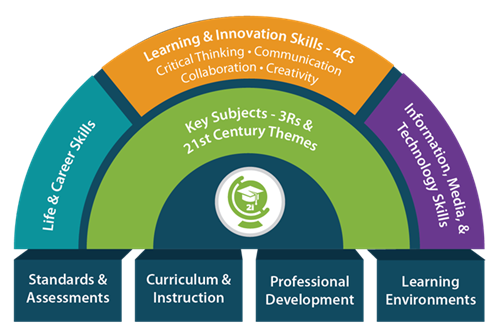
\includegraphics[width=70mm]{images/p21centuryskills.png}
        \end{center}
        \caption{Concept map figures}
        \label{intro::conceptmap}
    \end{figure}
    
    \begin{itemize}
        \item An external representation tool assist the learner in articulating 
        and maintaining shared focus during discourse \cite{Fischer2002FosteringTools,Suthers2006TechnologyCSCL,vanBoxtel2002CollaborativeDiscourse}
        \item A concept map has been widely used as a representational tool to facilitate group
        discussion, as well as to communicate complex ideas 
        \cite{Fischer2002FosteringTools,Gracia-Moreno2017CollaborativeWorkspaces,Suthers2006TechnologyCSCL,vanBoxtel2000CollaborativeKnowledge}
        \item A concept map is a graphical tool for organizing and representing knowledge which consists of concepts and relationships among these concepts to facilitate meaningful learning \cite{novak1984learning}.
        \item Previous studies posited that concept mapping has a positive effect on both students’ attitudes and learning achievements \cite{Basque2006CollaborativeTrends,Czerniak1998TheScience}.
    \end{itemize}
\end{frame}

\begin{frame}[allowframebreaks]{Collaborative concept mapping with KB approach}

    % add concept map figures
    \begin{figure}[tb]
        \begin{center}
            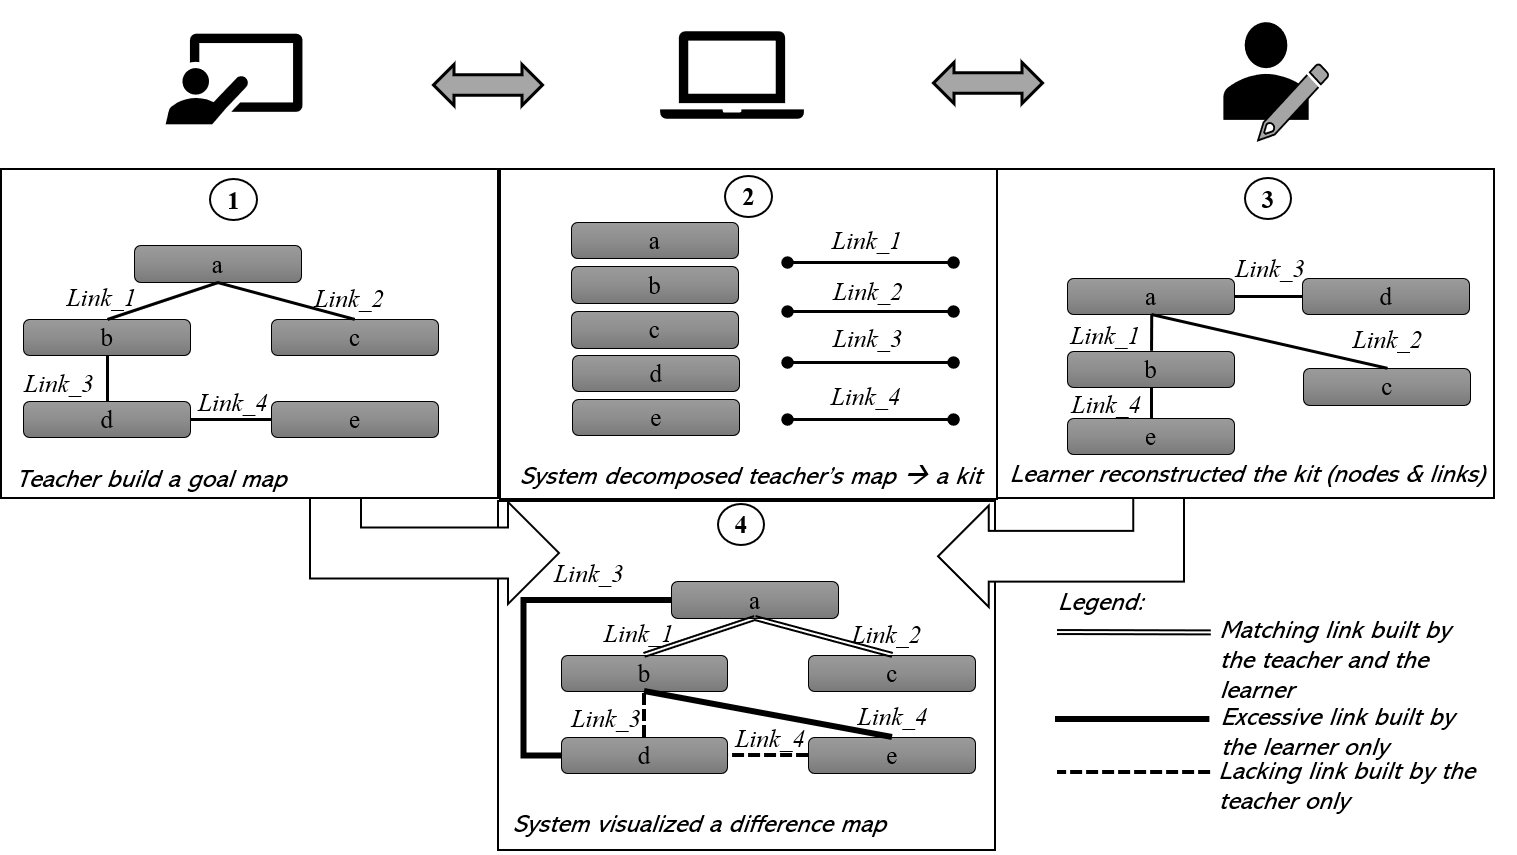
\includegraphics[width=70mm]{images/overview_kb.pdf}
        \end{center}
        \caption{Concept map figures}
        \label{intro::kbmap}
    \end{figure}
    
    \begin{itemize}
        \item The KB is a re-constructional closed-ended approach to concept mapping
        activity in which students construct a map based on predefined nodes and
        links extracted from an expert's map \cite{Hirashima2015,Hirashima2019ReconstructionalReconstruction}. 
        \item The KB approach enables teacher to confirm students' understanding
        of the information delivered by him/her. 
        \item Concept mapping activity with KB approach allow ones to externalize 
        their understanding on the perspective of other.
        \item Listening to other's and understand other's point of view are 
        key functions to collaborate effectively. 
        \item Therefore, we implemented the KB approach during 
        collaborative concept mapping to support communication and 
        build a shared knowledge between the group members.
    \end{itemize}
\end{frame}

\begin{frame}[allowframebreaks]{Challenges}
    \begin{itemize}
        \item Initial studies showed that the RKB approach promoted productive
        discussion between partners compared to the group without reconstruction
        and difference map-supported discussion
        \cite{Wunnasri2018ReciprocalUnderstanding}. 
        \item The RKB map also encouraged the pair of partners to understand each other based on the similarity
        score of the individual's map after discussion
        \cite{Wunnasri2018ReciprocalCollaboration}. 
        \item Their findings demonstrated that the RKB can be used to share understanding as preparation for
        collaboration. However, they have not evaluated the effect of applying
        this approach to collaborative knowledge building, so far. 
        \item \emph{Collaborative product evaluation} After following RKB activities, 
        whether or not high-quality group products could be achieved is still 
        a remaining question.  
        \item \emph{Students' perspective toward the activities} Applying new learning activity 
        in a practical classroom as a part of real teaching activity need to 
        consider the perspective of students. An evaluation regarding 
        students acceptance of this activity is as important as the learning product itself. 
        \item \emph{Group formation effect on collaboration} Researches suggest that 
        when forming a group, we need to consider several factors 
        such as similarity of individual knowledge, etc etc.
        To what extent, this factor would influence collaboration need to be investigated.
        By doing so, we could determine appropriate group settings. 
        \item \emph{Finding factor to consider for designing support function for collaboration}
        Which part of KB is a stronger predictor to estimate group product
        Whether similarity of individual knowledge or comprehension
        on partner's comprehension is a strong predictor to
        estimate the resulting product? 
    \end{itemize}
\end{frame}





\begin{frame}[allowframebreaks]{Research context}
\begin{itemize}
    \item Critical thinking in 21st century learning
    \item Critical thinking: What Every Person Needs to Survive in 
        a Rapidly Changing World
    \item CT definition: Critical thinking is disciplined, 
        self-directed thinking which exemplifies the 
        perfections of thinking appropriate to a 
        particular mode or domain of thought.
        (Paul, Elder 1990)
    \item A Brief Definition: Critical thinking is the art of 
        analyzing and evaluating thinking with a view to improving it
        (https://www.criticalthinking.org/pages/critical-thinking-where-to-begin/796)
    \item Critical thinking is, in short, self-directed,
        self-disciplined, self-monitored, and self-corrective 
        thinking. It requires rigorous standards of excellence 
        and mindful command of their use. It entails 
        effective communication and problem-solving 
        abilities, and a commitment to overcoming our 
        native egocentrism and sociocentrism.
    \item CT traits of mind: intellectual humility, 
        intellectual courage, intellectual empathy, intellectual 
        good faith (integrity), intellectual perseverance, 
        faith in reason, intellectual sense of justice.
    \item Intellectual empathy: recognizing the need to imaginatively
        put oneself in the place of others to genuinely 
        understand them
    \item These intellectual traits are interdependent. Each is best 
        developed while developing the others of well. 
    \item Effective collaboration is fueled by empathy—an awareness of
        others and an ability to detect their emotions and 
        understand their perspective. To come up with truly 
        innovative solutions requires new ideas.
\end{itemize}
\end{frame}

\note[itemize]{
\item Encouraging empathetic understanding to develop critical thinking
\item Critical thinking in 21st century learning
\item Why CT: Everyone thinks; it is our nature to do so. 
    But much of our thinking, left to itself, is biased, 
    distorted, partial, uninformed, or down-right prejudiced.
    Yet the quality of our lives and that of what we produce,
    make, or build depends precisely on the quality of our thought.
\item CT disposition (personal traits of mind)
\item Empathy as one of the disposition
\item Empathy: understanding one-self, understanding others, nonverbal empathy
\item Collaboration begins with empathy
\item Empathetic understanding for collaboration


}

\begin{frame}{Research motivations}

% \begin{itemize}
%   \item Peers do not learn because they are together, but because they perform
%         some activities which trigger specific learning mechanisms [1]
%   \item Various instructional strategies are designed to let learners to collaborate
%         (e.g. scripts, scenarios, visualization tool)
 %  \item Employing concept map during discourse has positively affected students 
 %        learning outcomes as well as their attitudes (e.g. motivation to learn, 
%         responsibility to participate [2, 3]
% \end{itemize}

\end{frame}



\begin{frame}{Problems during collaborative concept map}

\begin{itemize}
  \item Group more often neglected unshared resources [4]
  \item Difficulty in integrating different ideas while creating 
        a collaborative map [2]
  \item Some inaccurate ideas are never challenged and can become
        ingrained [2, 5]
\end{itemize}

\vskip 1cm

\begin{block}{The main question}
How to constructively built on individual ideas?
\end{block}

\end{frame}


\begin{frame}{Research questions}

\begin{itemize}
  \item aa
  \item bb
  \item cc
\end{itemize}

\end{frame}

\begin{frame}{Scope of research}
\begin{itemize}
    \item pair learning
    \item math subject
\end{itemize}
    
\end{frame}

\begin{frame}{Research roadmap}

\begin{itemize}
  \item aa
  \item bb
  \item cc
\end{itemize}

\end{frame}

